\documentclass{article}

\title{Simulating and Reconstructing X-Ray CT Projections}
\author{Reece Garthwaite}
\date{}

\usepackage{graphicx}
\usepackage{amsmath}
\usepackage{pythonhighlight}
\usepackage{float}
\usepackage{url}

\begin{document}
\maketitle

\begin{abstract}
I have chosen to simulate x-ray transmission through digital phantoms, using energy dependent attenuation from NIST data, to generate sinograms that I then reconstruct using simple back projection.
\end{abstract}

\section{Introduction}
Computed tomography (CT) scans are a form of medical imagery that uses x-rays to  create images of the body. CT scans reconstruct cross sectional images of the body from multiple projections of x-ray scans at a range of angles. This project aims to deepen my understanding of medical imaging techniques through the simulation and reconstruction of CT projections. 

This work particularly focuses on incorporating energy-dependent attenuation coefficients, derived from NIST data, to accurately model materials like bone and soft tissue, thereby allowing for the investigation of phenomena such as beam hardening.

\section{Methods}

\subsection{Background Physics}
\subsubsection{X-ray generation}
X-rays are produced when high kinetic energy electrons are accelerated towards a positive anode in a x-ray tube. Tungsten is a common choice for the anode (due to its high melting point and high atomic number). Electrons come close to nuclei of the target, causing a deceleration and change in direction, converting kinetic energy into a spectrum of electromagnetic radiation. Incident electrons can ionise the material, removing an electron from the anode. As the electron orbit vacancy gets filled by a orbital shell electron in a further out shell a photon is emitted. As orbital energies and their differences are unique in atoms, this leads to what we call "characteristic radiation".
\cite{Tafti}

\begin{figure}
  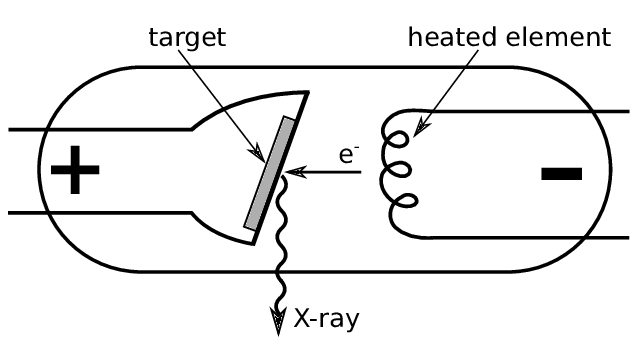
\includegraphics[width=\linewidth]{xray_tube.png}
  \caption{Schematic of a X-ray tube}
  \label{fig:X-ray tube}
\end{figure}

Figure \ref{fig:X-ray tube} \cite{Mason} shows a diagram of a x-ray tube . Which helps to visualise the origin of the x-ray spectrum as electrons are emitted via thermionic emission and then accelerated toward a positively charged anode, where their interactions with the target produce both bremsstrahlung and characteristic radiation.

\subsubsection{Attenuation of X-rays}
As x-rays pass through matter, they are attenuated according to the Beer-Lambert law: 
\begin{equation} \label{bl}
I(E) = I_0 \cdot e^{-\mu(E) x}
\end{equation}

Where:
\begin{itemize}
  \item I = transmitted intensity of radiation after passing through the material
  \item $I_0$ : Initial intensity
  \item $\mu$ : Linear attenuation coefficient
  \item $x$ : Thickness of material
\end{itemize}

I have included  $\mu$ to be energy dependent as this is what is observed in experiments, and allows us to look for an interesting phenomenon known as beam hardening. I calculate $\mu$ using:
\begin{equation} \label{linearatt}
\mu(E) = \left(\frac{\mu}{\rho}\right) \cdot \rho
\end{equation}
Where $\left(\frac{\mu}{\rho}\right)$ is the mass attenuation coefficient from NIST \cite{nistXRayMass}

\subsection{Investigating Beam Hardening}
Beam hardening occurs during x-ray attenuation as higher energy (hard) X-rays penetrate dense materials more effectively than the low energy (soft) X-rays. This has the effect of shifting the peak of the bremsstrahlung radiation towards higher energies. Beam hardening cannot occur for monochromatic X-rays, as the average energy will not change, so we can predict that the characteristic radiation will not harden.
I used spekpy, a dedicated x-ray spectrum simulation toolkit, and matplotlib to generate a typical spectra from a Tungsten x-ray tube and plot for energies upto 150 keV. I used a 2mm Aluminium filter to remove low energy, non-diagnostic x-rays. We can use spekpys built in filter function for this but will also write our own filtering code shortly.

\begin{figure}
	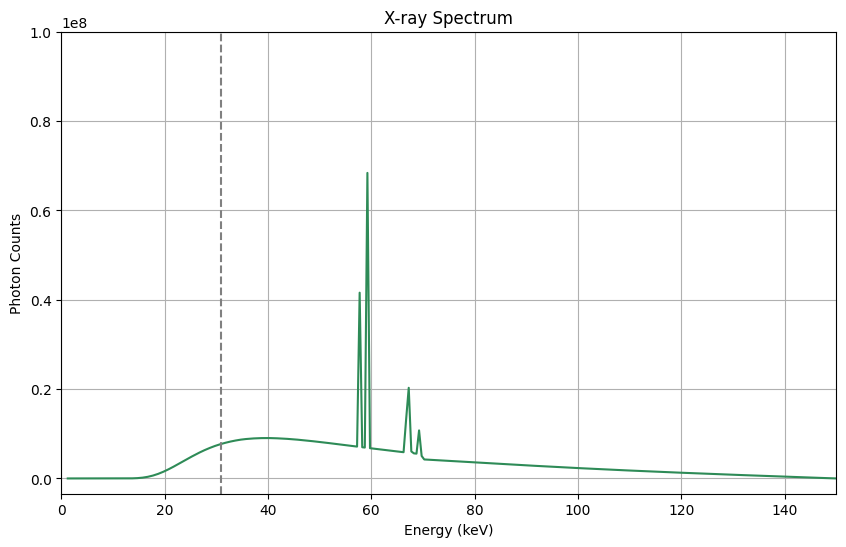
\includegraphics[width=\linewidth]{typicalxrayspectra.png}
	\caption{X-ray Spectrum from a x-ray tube with a Tungsten target}
  \label{fig:basespectra}
\end{figure}

In Figure \ref{fig:basespectra} we can see the sharp characteristic peaks that correspond to Tungsten. Writing code for filtering using NIST data and interpolation to fit the number of data points required., 

\begin{python}
import pandas as pd
from scipy.interpolate import interp1d

# Load csv
bone_data = pd.read_csv("bone.csv", names=["Energy_MeV", "Mu_Rho"], header=None)#

# Convert energy to KeV
bone_data["Energy_KeV"] = bone_data["Energy_MeV"] * 1000

# Average out duplicates by grouping
bone_data = bone_data.groupby("Energy_KeV", as_index=False).mean()

# Convert to linear attenuation (mu = mu/rho * rho)
bone_density = 1.85  # g/cm^3
bone_data["Mu"] = bone_data["Mu_Rho"] * bone_density  # [cm^-1]
mu = bone_data["Mu"].to_numpy()

# Create interpolation function for attenuation coefficients
mu_interp = interp1d(bone_data["Energy_KeV"], bone_data["Mu"], bounds_error=False, fill_value="extrapolate")

mu_at_spectrum_energies = mu_interp(energies)

thickness_cm = 0.5
I0 = s.get_spk()

I_filtered = I0 * np.exp(-mu_at_spectrum_energies * thickness_cm)
\end{python}

\begin{figure}[H]
	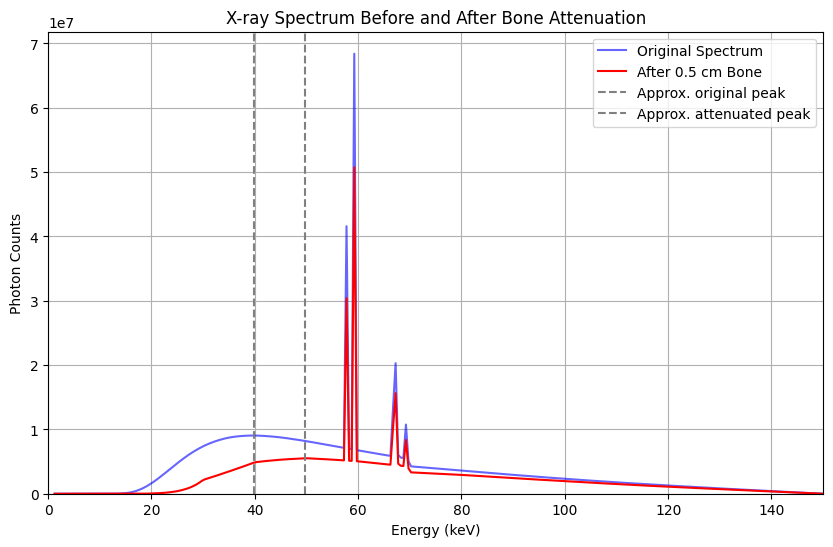
\includegraphics[width=\linewidth]{beamhardening.png}
	\caption{Comparing X-ray spectra before and after passing through 0.5cm of bone}
  \label{fig:beamhardening}
\end{figure}

Figure \ref{fig:beamhardening} shows beam hardening on the X-ray spectrum. The lower-energy (soft) x-rays are preferentially attenuated, resulting in a spectrum that is skewed toward higher energies. Lower-energy photons are absorbed more readily than high-energy ones. As a result, the transmitted spectrum becomes "hardened," with its average energy increasing. We also don't see any hardening for the monochromatic peaks, as expected. 

Beam hardening is significant in image reconstruction, as it may result in characteristic artefacts. CT beam hardening artefacts are known as: streaking artefacts, where dark bands appear between dense structures, and cupping artefacts, where the center of a homogeneous object appears less attenuating than the periphery \cite{Murphy_2016}.

\subsection{Phantoms and Sinograms}
\subsubsection{Generating Phantoms}
In medical scans, phantoms are used as stand-ins for human tissues to ensure that systems and methods are working correctly. One common such phantom is the Shepp-Logan phantom \cite{Shepp_Logan_1974}. The Shepp-Logan phantom is a standard benchmark for CT reconstruction algorithms due to its complex structure that still models real world conditions.

\begin{figure}.
	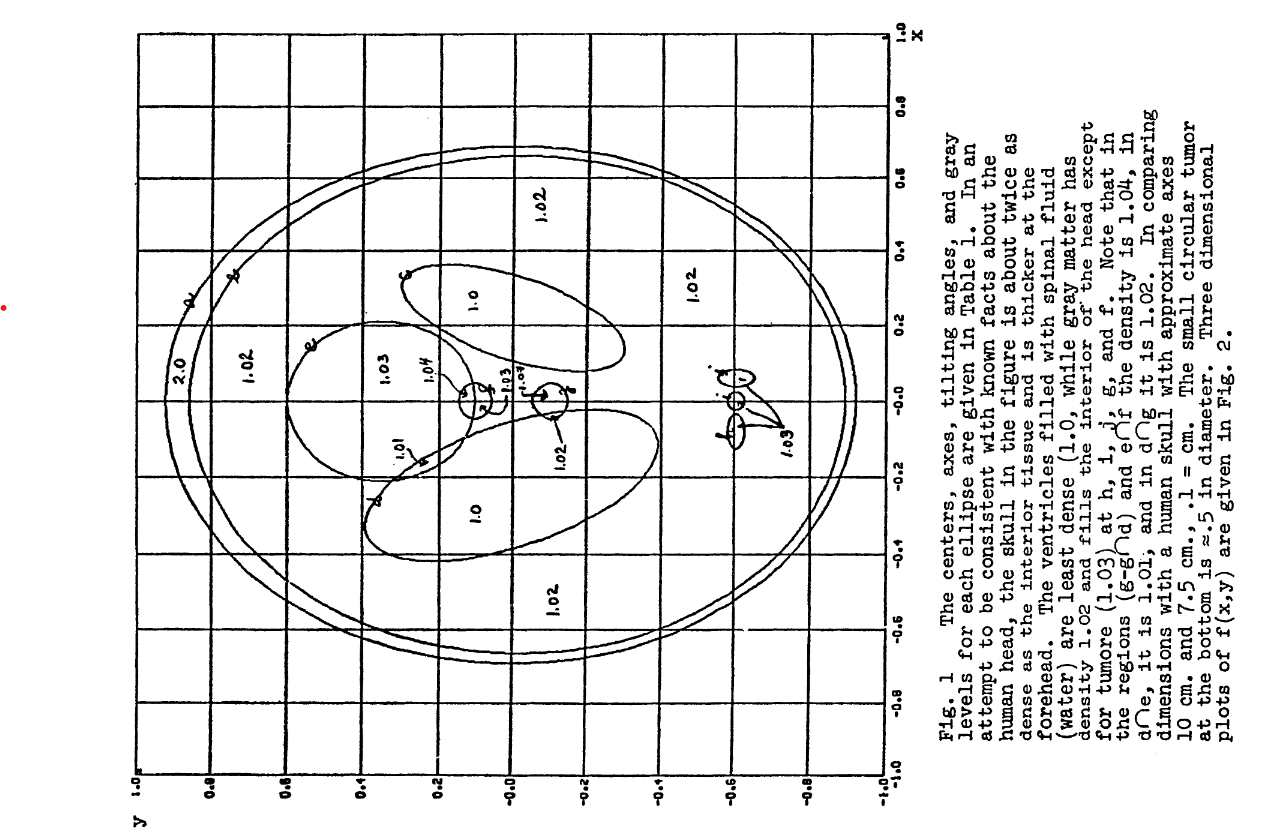
\includegraphics[width=\linewidth]{shepplogan.png}
	\caption{Shepp-Logan head phantom image}
	\label{fig:shepplogan}
\end{figure}

Using Jan Hrach's python code, \cite{phantom_py}, I can recreate the Shepp-Logan phantom with constant attenuation coefficients.

Another phantom I created was a simple circle of bone surrounded by a larger circle of soft tissue. This was an easy way to test using the energy dependent attenuation coefficients. The $circlemask$ function is use to define circular regions on the phantom, which can then be assigned with properties for different materials. Using a phantom with simplified geometry allowed for clearer observation of attenuation characteristics.

\begin{python}
def circlemask(radii, centre_x, centre_y, width, height):
    x, y = np.ogrid[:width, :height]
    mask = (x-centre_x)**2 + (y-centre_y)**2 <= radii**2
    return mask
   
width, height = 180,180
s = sp.Spek(kvp=150,th=12)
energies = s.get_k()
# Load each material from a csv file
mu_bone = load_mu_data(r"code\bone.csv", density=1.85, energy_range_KeV=energies)
mu_tissue = load_mu_data(r"code\soft_tissue.csv", density=1.06, energy_range_KeV=energies)
E=len(energies)

phantom = np.zeros((height, width, E))
bone_mask = circlemask(10,width//2,height//2,width,height)
thigh_mask=circlemask(40,width//2,height//2,width,height)

# Background
phantom[:, :, :] = 0  # broadcast over all pixels

# Thigh region
phantom[thigh_mask, :] = mu_tissue

# Bone region
phantom[bone_mask, :] = mu_bone
\end{python}

Using matplotlib to display these phantoms:

\begin{figure}[H]
	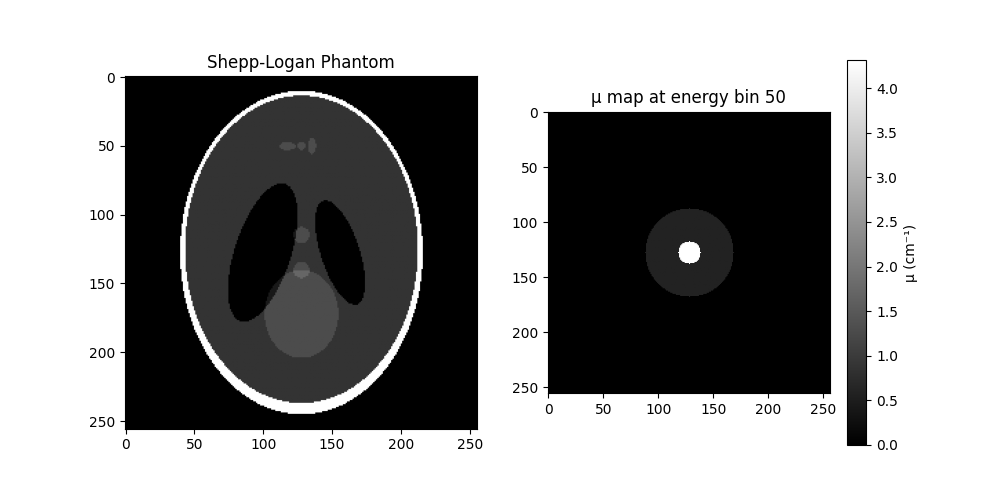
\includegraphics[width=\linewidth]{simplephantom.png}
	\caption{Left: Shepp-Logan phantom. Right: Circular phantom with central bone inclusion ($\mu$ map at energy bin 50).}
	\label{fig:phantoms}
\end{figure}

\subsubsection{Sinograms}
In order to think about image reconstruction we need to think about projections. A projection in CT scans represents the total attenuation of x-rays along a specific path of the object. At an angle $\theta$, the parallel beam geometry represents a new coordinate system $(r, s)$ in which the intensity profile $I_\theta (r)$ is measured. 
All points $(x,y)$ satisfy $r = x \cos(\theta) + y \sin(\theta)$, and $s$ is the parametric variable along the ray line.

$$\begin{pmatrix} r \\ s \end{pmatrix} = R \begin{pmatrix} x \\ y \end{pmatrix} = \begin{pmatrix} \cos\theta & \sin\theta \\ -\sin\theta & \cos\theta \end{pmatrix} \begin{pmatrix} x \\ y \end{pmatrix}$$

Conversely,
$$\begin{pmatrix} x \\ y \end{pmatrix} = R^T \begin{pmatrix} r \\ s \end{pmatrix} = \begin{pmatrix} \cos\theta & -\sin\theta \\ \sin\theta & \cos\theta \end{pmatrix} \begin{pmatrix} r \\ s \end{pmatrix}$$

Using parallel beam geometry and a fixed angle $\theta$, the measured intensity at position $r$ is the integrated mass attenuation  along $L_{(r,\theta)}$:

\begin{align}
I_{\theta}(r) &= I_0 \cdot \exp\Bigl({-\int\limits_{L_{(r,\theta)}} \mu (x,y) ds} \Bigr) \\
& = I_0 \cdot \exp\Bigl({-\int\limits_{L_{(r,\theta)}} \mu \left(r \cos(\theta) - s \sin(\theta),r \sin(\theta) + s \cos(\theta)\right) ds} \Bigr) 
\end{align}

Each Intensity profile $I_\theta (r)$ is transformed into an attenuation profile $p_\theta (r)$:

\begin{align}
p_\theta (r) = - \ln \frac{I_\theta (r)}{I_0} = -\int\limits_{L_{(r,\theta)}} \mu \left(r \cos(\theta) - s \sin(\theta),r \sin(\theta) + s \cos(\theta)\right) ds
\end{align}

\bibliography{References}
\bibliographystyle{ieeetr}
\end{document}
